\section{Вычислительный эксперимент}
\label{sec:Chapter4} \index{Chapter4}

Цель экспериментов~--- проверить предсказания теорем~\ref{thm:beta}
и~\ref{thm:loop} в управляемой среде, где каждый компонент контура поддаётся
точному контролю, а затем убедиться в переносимости выводов на реальные данные.
Синтетическая постановка позволяет изолировать исследуемый эффект от посторонних
факторов~--- неоднородности поведения, шума измерений, случайностей обработки.
Такой подход близок к симуляционным средам для рекомендательных систем и
моделям с синтетической обратной связью, но здесь симулятор используется не для обучения
политики, а для проверки механизма петли~\cite{ie2019,
wang2021generativeFeedback, afsar2022rlSurvey}.

\subsection{Постановка эксперимента}
\label{subsec:exp_setup}

Симулятор воспроизводит один шаг контура из раздела~\ref{subsec:one_step}:
формирование списка top-$L$, отклик по модели следования, запись логов,
дрейф~\eqref{eq:drift}, переобучение раз в $T_{\mathrm{ret}}$ шагов и подсчёт
метрик. Рекомендательная модель~--- многослойный персептрон (MLP), получающий
конкатенацию представлений пользователя и объекта, со скрытым слоем ReLU,
сигмоидным выходом и обучением методом Adam по бинарной кросс-энтропии; в части экспериментов
используется матричная факторизация $f=\sigma(u^\top M v+b)$. Нейросетевая
оценка релевантности выбрана как стандартная современная альтернатива классическим
матрично-факторизационным моделям~\cite{he2017}. Популяция
порождается смесью $K$ гауссиан; на каждом шаге доля наименее активных
пользователей заменяется новыми, сгенерированными из текущего распределения.
Тем самым симулятор снимает допущение о неизменном составе когорты,
использованное в теоретическом анализе: идентичность части пользователей между
соседними шагами не сохраняется.

В практической выдаче объект, уже показанный пользователю, обычно исключается из
его последующих списков. В основной конфигурации симулятора используется фильтр
\texttt{seen\_filter}; доступный каталог пользователя исключает объекты, для
которых зарегистрировано предыдущее взаимодействие. Это является приближением к
продуктовому правилу фильтрации всех прошлых экспозиций, поскольку симулятор
регистрирует в матрице не каждый показ, а наблюдаемый отклик. В отдельных
диагностических запусках фильтр отключается, когда требуется изолировать
геометрию закона выдачи от исчерпания доступного каталога; такие запуски
оговариваются отдельно.

Для разделения механизмов сравниваются четыре режима, отличающиеся обработкой
переобучения и силой контура (таблица~\ref{tab:regimes}). Базовая конфигурация:
$d=8$, $N=M=300$, $K=3$, $L=10$, $T=100$, $T_{\mathrm{ret}}=10$, замена $5\%$ за
шаг, $\alpha=0{,}7$, $\beta=0{,}005$, межкластерное расстояние $5{,}0$; метрики
усредняются по $5$ независимым запускам. Исходный код доступен в
репозитории\footnote{Директория \texttt{code/} проекта.}.

\begin{table}[H]
    \caption{Режимы сравнения}
    \label{tab:regimes}
    \centering
    \begin{tabular}{ll}
        \toprule
        Режим & Поведение \\
        \midrule
        \texttt{closed\_loop}  & переобучение на собственных логах, $\alpha>0$ \\
        \texttt{static}        & $\alpha>0$, модель заморожена \\
        \texttt{fresh\_oracle} & переобучение на истинных вероятностях отклика \\
        \texttt{no\_influence} & $\alpha=0$, отклик только по истинной вероятности \\
        \bottomrule
    \end{tabular}
\end{table}

\subsection{Универсальность стягивания разнообразия}
\label{subsec:exp_universal}

Согласно Теореме~\ref{thm:beta} и следствию~\ref{cor:universal}, стягивание
разнообразия определяется силой дрейфа $\beta$ и не зависит от режима
переобучения. Решающую проверку даёт варьирование $\beta$ при прочих
фиксированных параметрах. Тем самым проверяется более сильное утверждение, чем в
работах о деградации из-за повторного переобучения: если $\beta>0$, стягивание
может возникать и без обновления модели~\cite{jiang2019,
barlacchi2026diversityParadox}.

\begin{figure}[H]
    \centering
    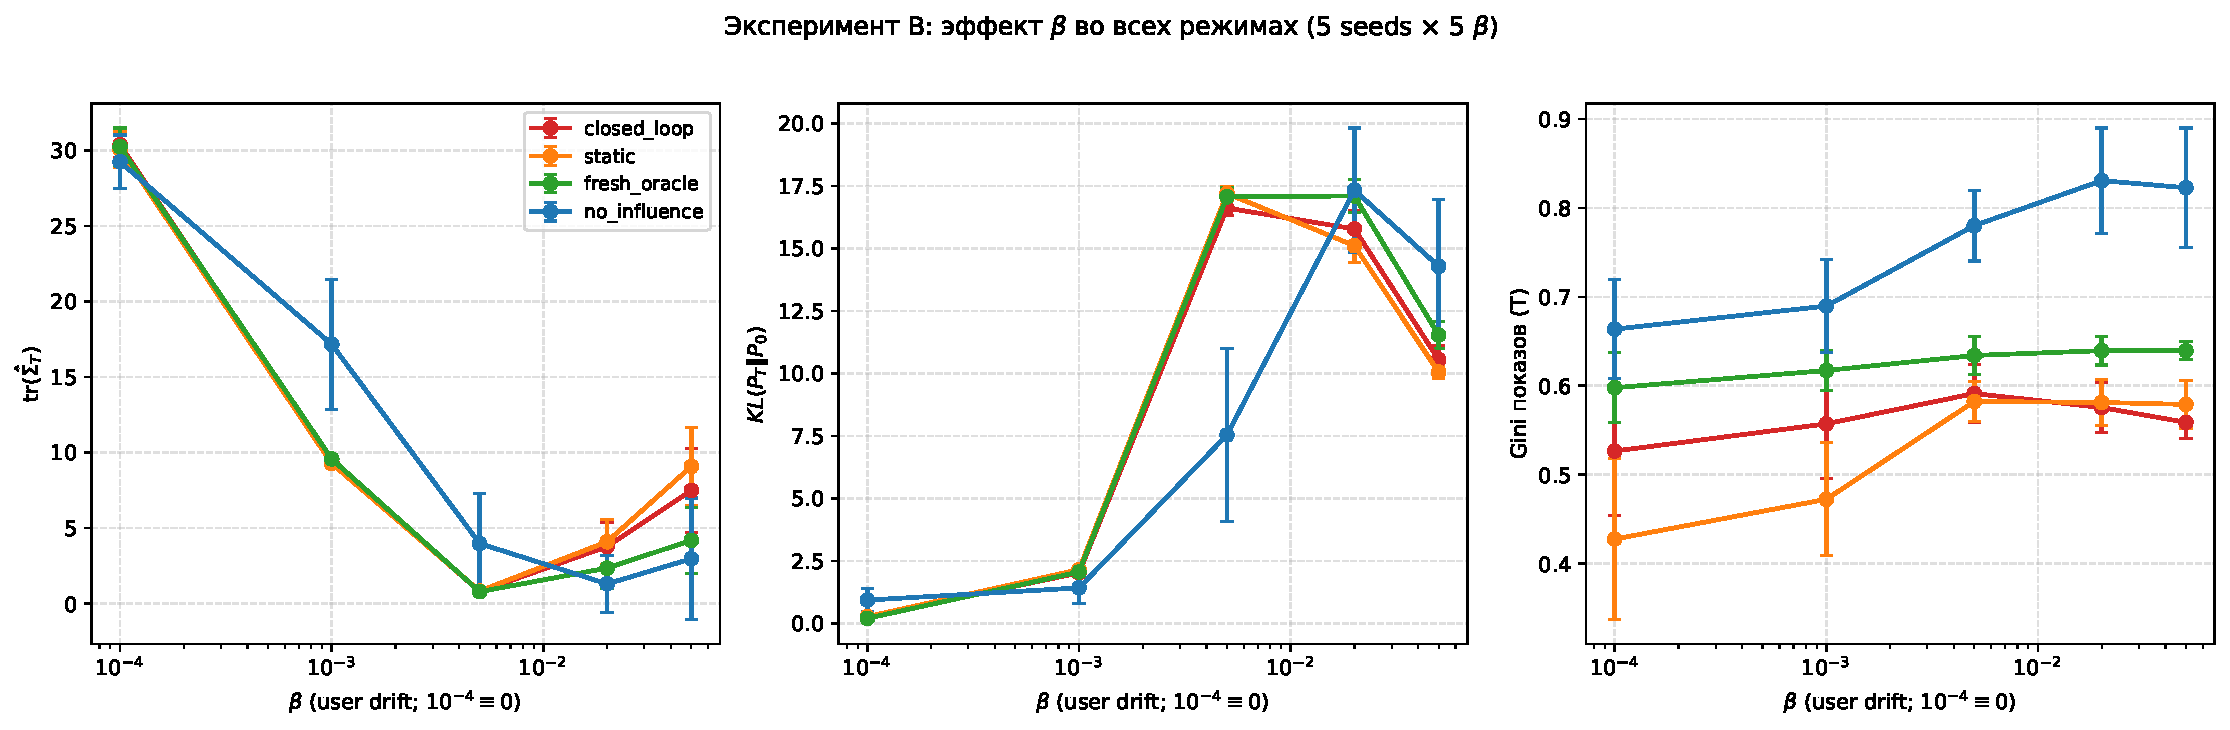
\includegraphics[width=0.85\textwidth]{figures/diagnostic/DIAG_B_beta_sweep_v2}
    \caption{Остаточное разнообразие $\operatorname{tr}\hat\Sigma$ после $T$ шагов
    как функция силы дрейфа $\beta$ для четырёх режимов. При $\beta=0$ стягивания
    нет ни в одном режиме; при $\beta>0$ оно наступает одинаково во всех режимах с
    $\alpha>0$, что подтверждает следствия~\ref{cor:no_beta}
    и~\ref{cor:universal}.}
    \label{fig:beta_sweep}
\end{figure}

При $\beta=0$ след ковариации сохраняется на уровне $\operatorname{tr}
\hat\Sigma\approx30$ во всех режимах, включая режим петли (рис.~\ref{fig:beta_sweep}),
что прямо подтверждает следствие~\ref{cor:no_beta}. При $\beta=0{,}005$
стягивание достигает максимума ($\operatorname{tr}\hat\Sigma\approx0{,}8$) во
всех режимах с $\alpha>0$. Дополнительный эксперимент со статической моделью при
варьировании $\alpha$ показывает, что уже при $\alpha\ge0{,}4$ стягивание
достигает уровня петли, то есть переобучение не является его источником.

\begin{figure}[H]
    \centering
    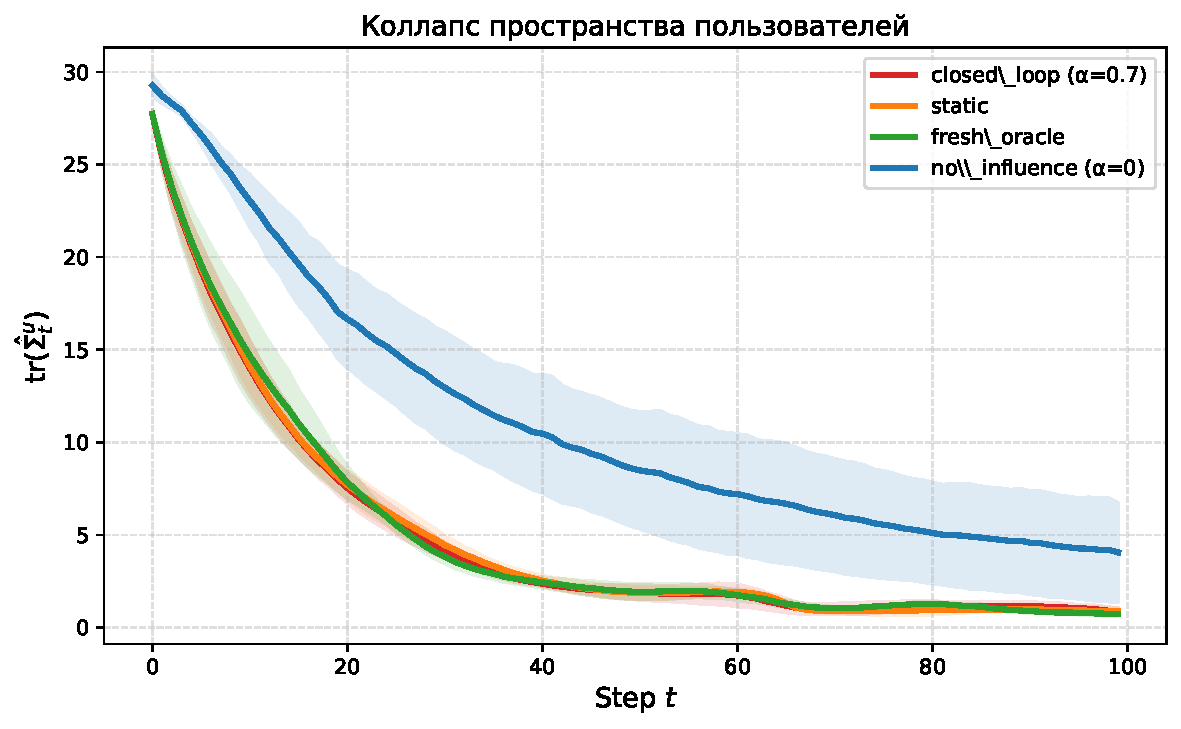
\includegraphics[width=\textwidth]{figures/H1_H3_trace_sigma}
    \caption{Динамика следа ковариации $\operatorname{tr}\hat\Sigma_t$ по четырём
    режимам. Стягивание наступает во всех режимах с дрейфом; режим без следования
    рекомендациям \texttt{no\_influence} стягивается слабее за счёт большего
    разброса показанного.}
    \label{fig:h1h3_trace}
\end{figure}

Численные итоги приведены в таблице~\ref{tab:h1h3}. Стягивание следа ковариации в
режиме петли составляет $-96{,}9\%$, в режиме \texttt{no\_influence}~---
$-86{,}1\%$; режимы \texttt{static} и \texttt{fresh\_oracle} дают близкий к петле
результат ($-96{,}8\%$ и $-97{,}4\%$), что согласуется со
следствием~\ref{cor:universal}: закон убывания общий для всех режимов с дрейфом.

\begin{table}[H]
    \caption{Итоговые метрики после $T=100$ шагов (среднее по $5$ запускам)}
    \label{tab:h1h3}
    \centering
    \begin{tabular}{lccc}
        \toprule
        Режим & $\mathrm{KL}(P_T\Vert P_0)$ & $\operatorname{tr}\hat\Sigma_T$ & $\Delta\operatorname{tr}$, \% \\
        \midrule
        \texttt{closed\_loop}  & $16{,}88$ & $0{,}865$ & $-96{,}9$ \\
        \texttt{static}        & $17{,}25$ & $0{,}878$ & $-96{,}8$ \\
        \texttt{fresh\_oracle} & $16{,}95$ & $0{,}723$ & $-97{,}4$ \\
        \texttt{no\_influence} & $\phantom{0}7{,}31$ & $4{,}06$ & $-86{,}1$ \\
        \bottomrule
    \end{tabular}
\end{table}

\subsection{$K$-модальная структура эхо-камер}
\label{subsec:exp_kmodal}

Теорема~\ref{thm:beta} применяется к каждому кластеру отдельно, поэтому при
$K>1$ ожидается формирование $K$ независимых зон стягивания при сохранении
межкластерного зазора. Гипотеза проверяется на сетке значений числа кластеров
$K\in\{1,2,4\}$ и межкластерного расстояния.

\begin{figure}[H]
    \centering
    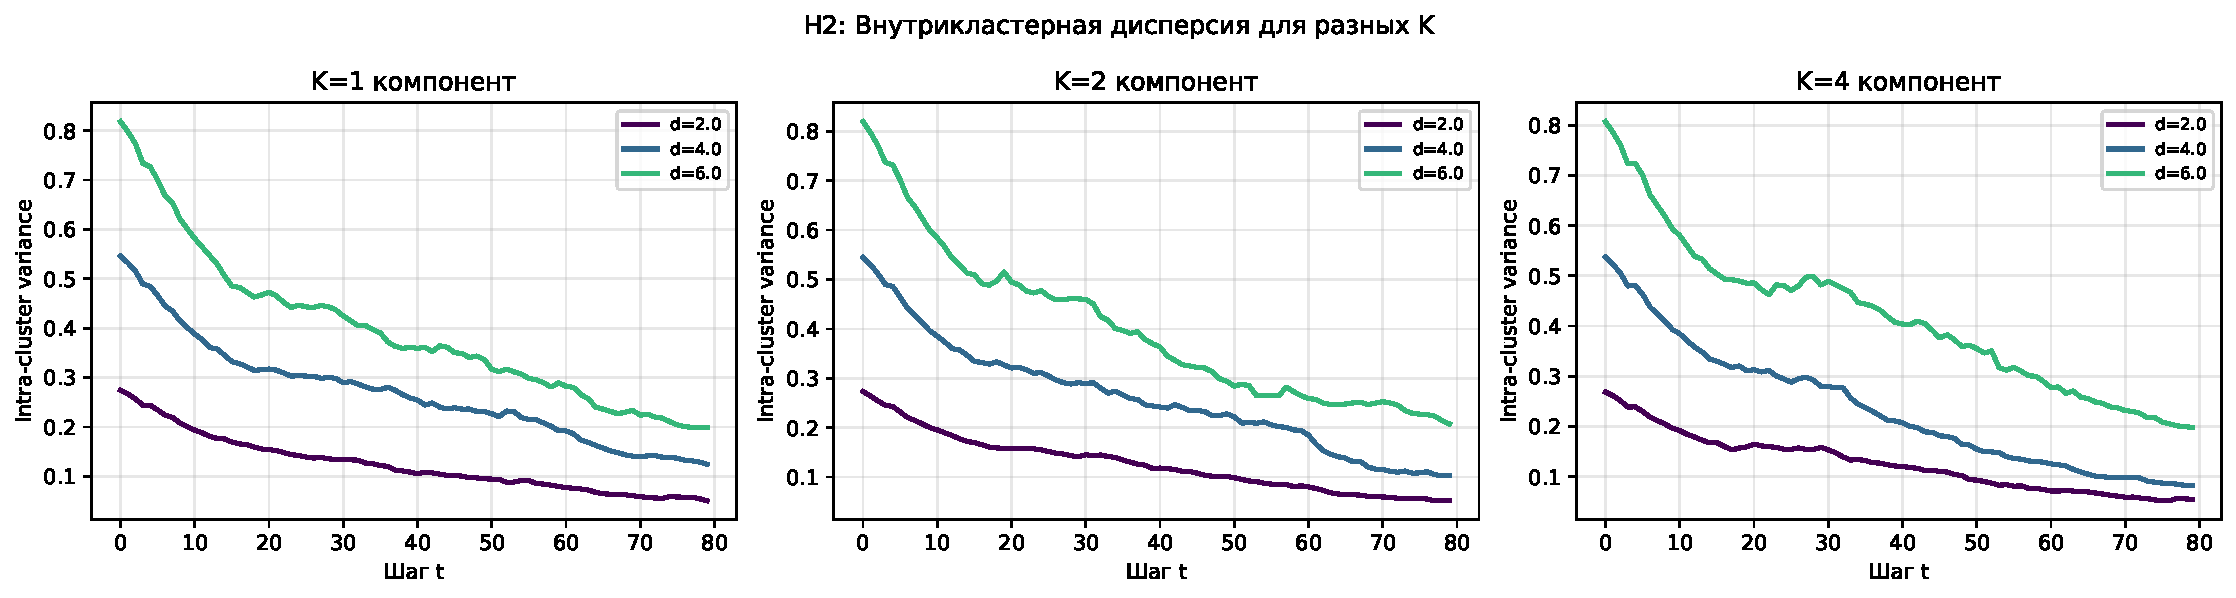
\includegraphics[width=\textwidth]{figures/H2_intra_cluster_variance}
    \caption{Внутрикластерная дисперсия во времени при $K\in\{1,2,4\}$ и трёх
    значениях межкластерного расстояния. Дисперсия убывает на $77$--$85\%$,
    быстрее при большем $K$.}
    \label{fig:h2_intra}
\end{figure}

Внутрикластерная дисперсия убывает на $77\%$ при $K=1$, на $81\%$ при $K=2$ и на
$85\%$ при $K=4$ (рис.~\ref{fig:h2_intra}); коэффициент силуэта при этом не
деградирует ($0{,}634\to0{,}677$ при $K=4$), то есть кластеры уплотняются, но не
сливаются. Скорость стягивания растёт с $K$: чем теснее объекты к пользователям
своего сегмента, тем эффективнее дрейф концентрирует эмбеддинги. Качественная
картина показана на PCA-снимках (рис.~\ref{fig:t3_pca}): облака сжимаются к
центроидам при сохранении расстояния между ними.

\begin{figure}[H]
    \centering
    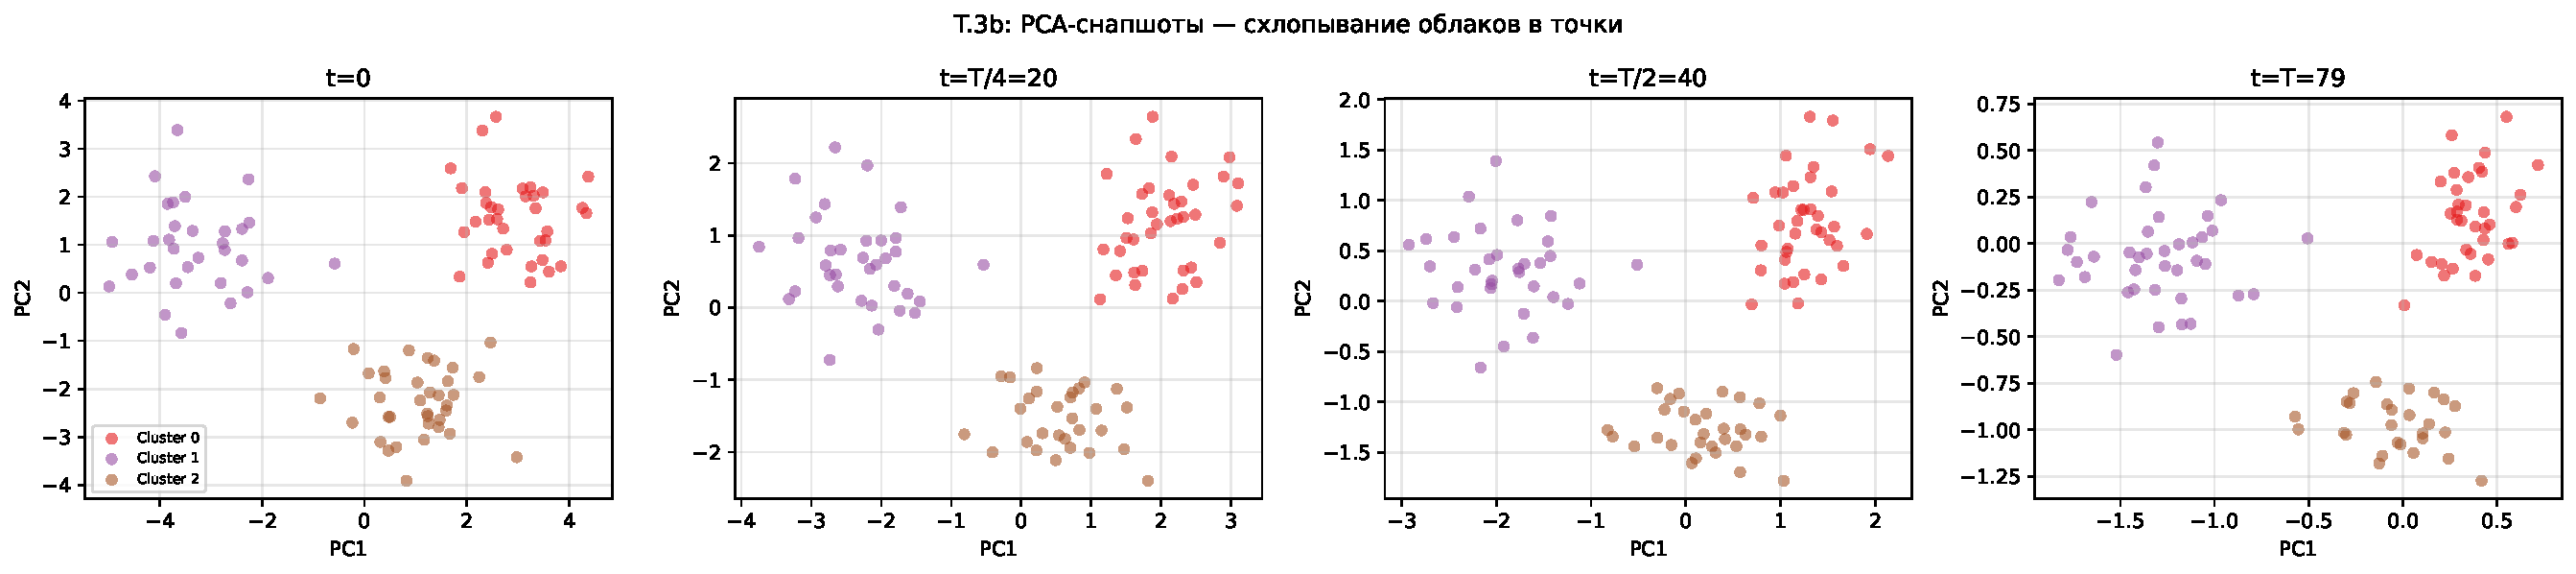
\includegraphics[width=\textwidth]{figures/T3_pca_snapshots}
    \caption{Снимки эмбеддингов (метод главных компонент) в моменты $t\in\{0,
    T/4, T/2, T-1\}$ при $K=3$; цвет~--- кластер. Стягивание персонализации внутри
    кластеров при сохранении межкластерного разделения.}
    \label{fig:t3_pca}
\end{figure}

\subsection{Геометрия стягивания}
\label{subsec:exp_geometry}

Ряд проверок уточняет геометрию предельного режима, предсказанного
Теоремой~\ref{thm:beta}. Спектральный радиус $\lambda_{\max}(\hat\Sigma_k)$
монотонно убывает для всех кластеров; для $23$ независимых начальных
распределений все траектории среднего следа монотонно убывают к нулю, что
подтверждает глобальность аттрактора. Внутрикластерный индекс Жаккара рекомендаций
растёт с $0{,}50$ до $0{,}86$ ($+71\%$): к концу горизонта пользователи одного
кластера получают почти одинаковые списки.

\begin{figure}[H]
    \centering
    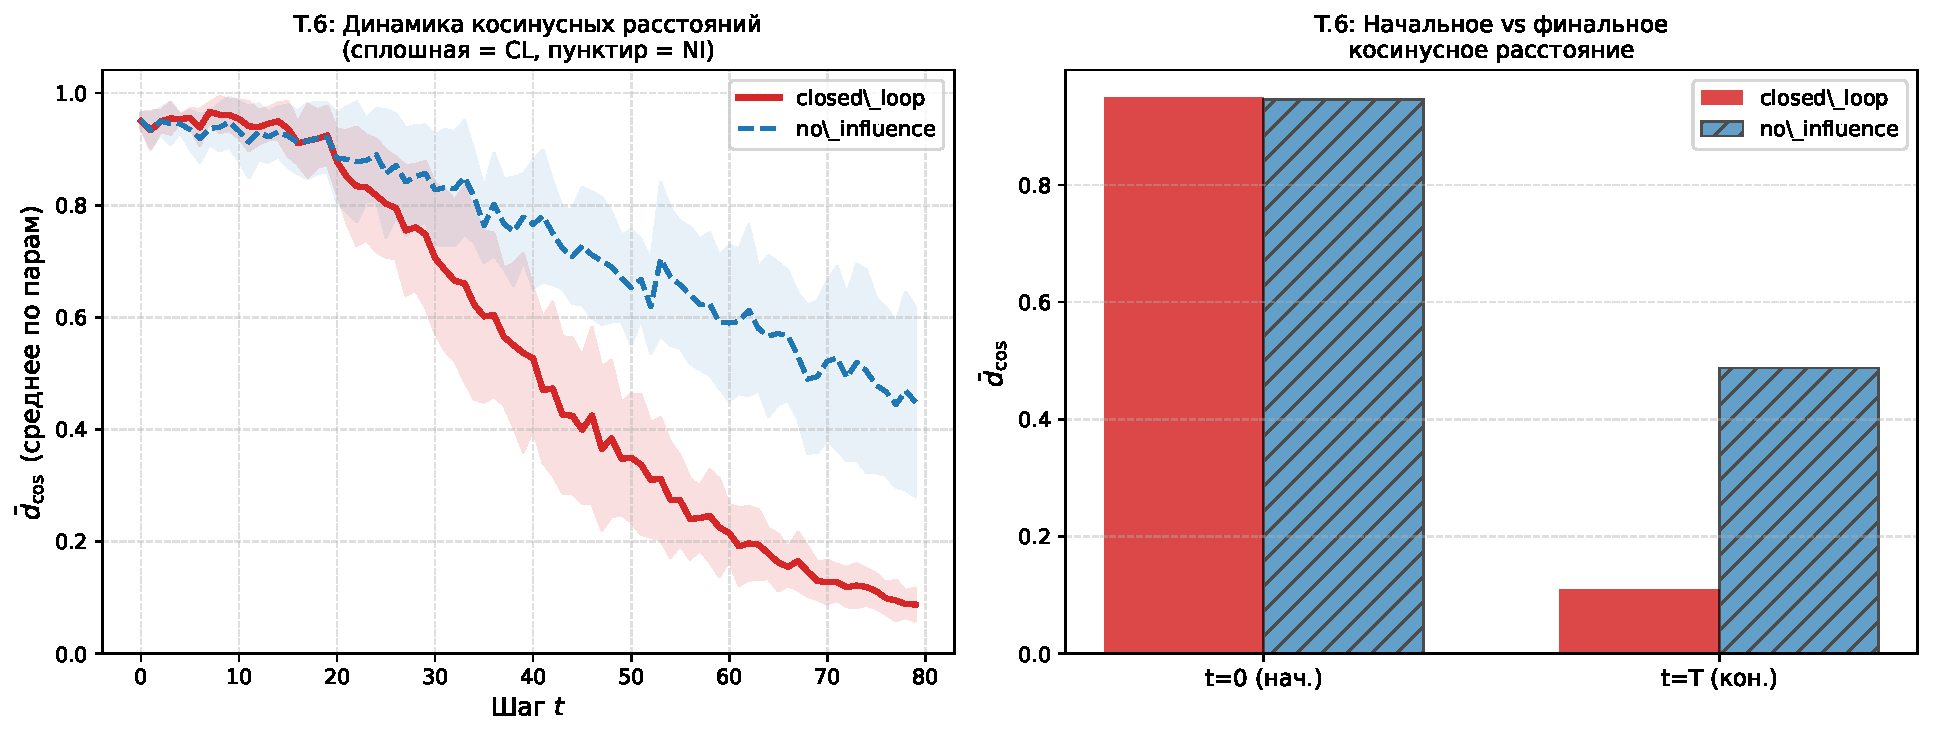
\includegraphics[width=0.9\textwidth]{figures/T6_cosine_distances}
    \caption{Среднее попарное косинусное расстояние между пользователями. В
    режиме петли эмбеддинги становятся почти коллинеарны ($d_{\cos}\approx0{,}11$),
    тогда как в \texttt{no\_influence} сохраняется существенное угловое
    разнообразие ($d_{\cos}\approx0{,}49$).}
    \label{fig:t6_cosine}
\end{figure}

Среднее попарное косинусное расстояние (рис.~\ref{fig:t6_cosine}) убывает в петле
в $4{,}4$ раза сильнее, чем в контрольном режиме, то есть кластер схлопывается к
почти одномерному подпространству вдоль направления доминирующего объекта.
Анализ фрагментации (рис.~\ref{fig:t7_frag}) показывает, что доля межкластерной
дисперсии $\eta^2$ в петле растёт ($0{,}33\to0{,}46$): аудитория всё чётче
распадается на изолированные сегменты.

\begin{figure}[H]
    \centering
    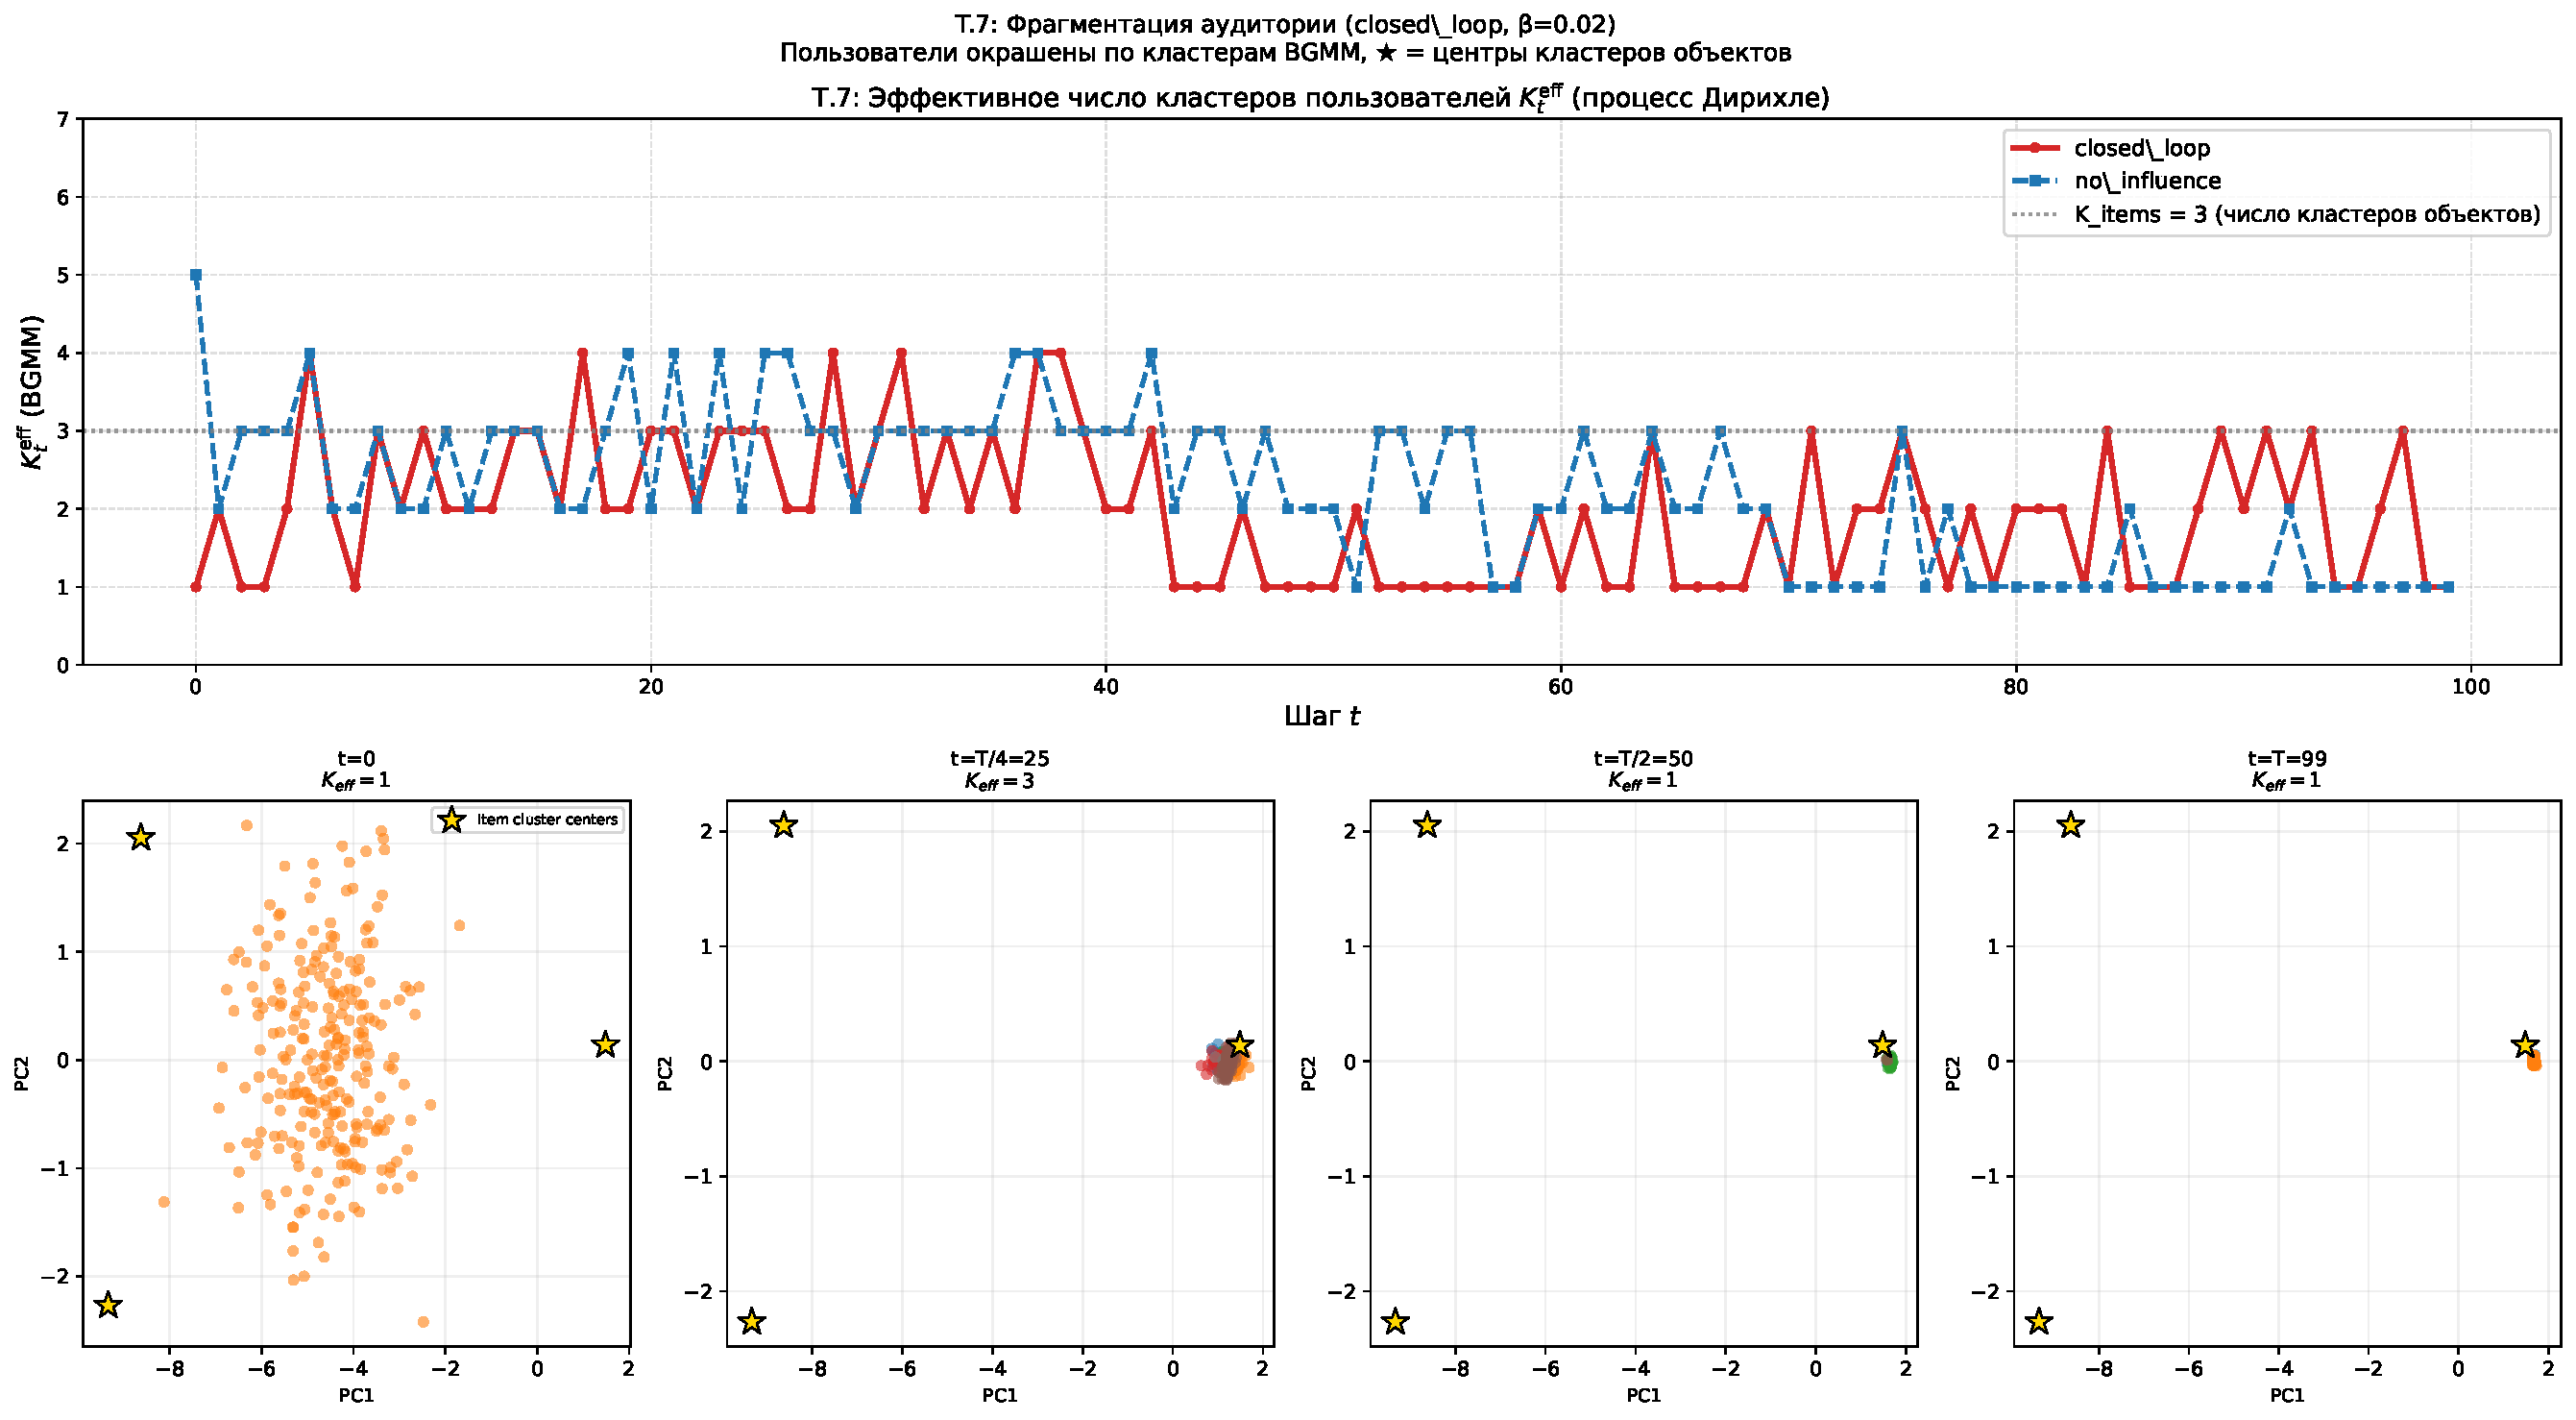
\includegraphics[width=0.8\textwidth]{figures/T7_fragmentation_dpmm}
    \caption{Доля межкластерной дисперсии $\eta^2$ во времени. В режиме петли рост
    выражен сильнее ($0{,}33\to0{,}46$), чем в \texttt{no\_influence}
    ($0{,}36\to0{,}40$): популяция фрагментируется на изолированные сообщества.}
    \label{fig:t7_frag}
\end{figure}

\subsection{Фазовая диаграмма стягивания}
\label{subsec:exp_phase}

Теорема~\ref{thm:beta} предсказывает, что граница стягивания определяется
произведением силы следования и активности. На сетке $8\times8$ по
$(\alpha,\rho)$ ($192$ запуска) измерялась остаточная доля дисперсии.

\begin{figure}[H]
    \centering
    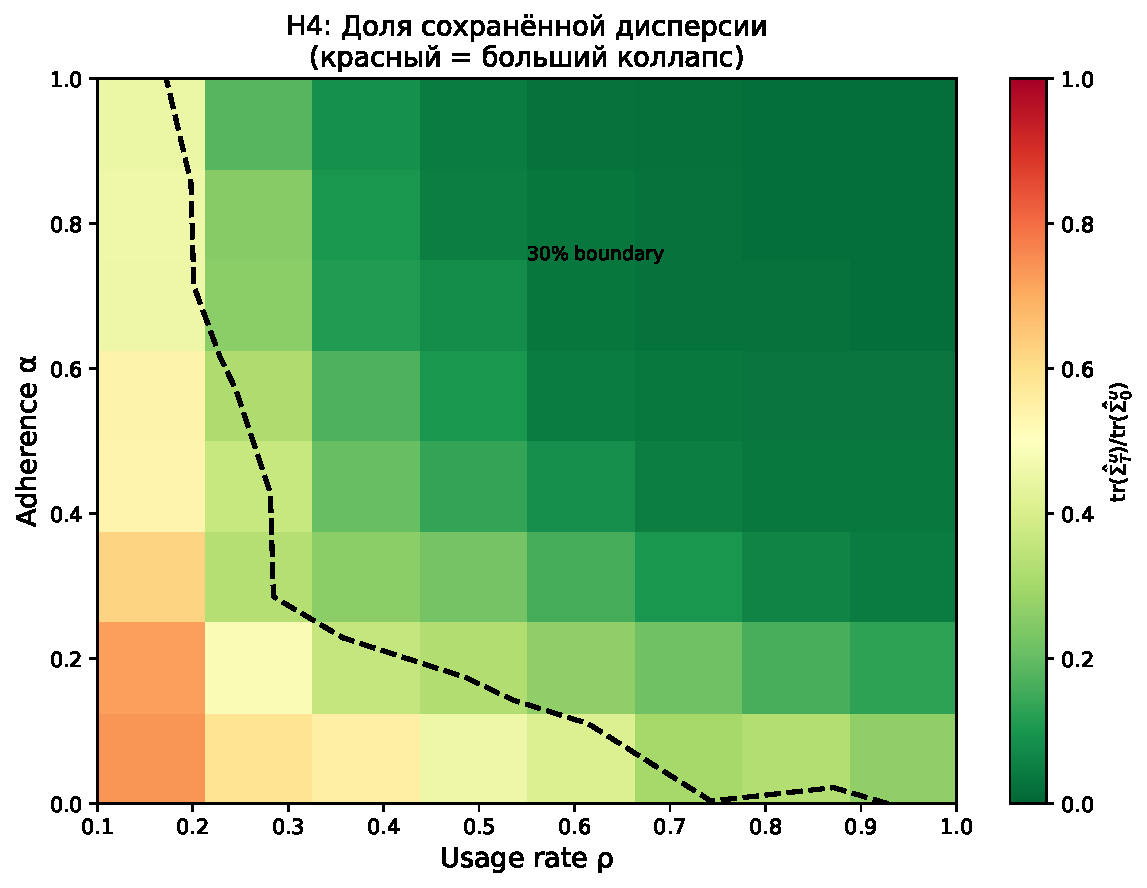
\includegraphics[width=\textwidth]{figures/H4_phase_diagram}
    \caption{Фазовая диаграмма остаточной доли дисперсии в координатах (сила
    следования $\alpha$, активность $\rho$). Граница стягивания определяется
    произведением $\alpha\cdot\rho$: чем оно больше, тем полнее стягивание.}
    \label{fig:h4_phase}
\end{figure}

При $\rho=1$ остаточная доля монотонно убывает с $0{,}268$ при $\alpha=0$ до
$0{,}018$ при $\alpha=1$ (рис.~\ref{fig:h4_phase}). Линии уровня диаграммы близки
к гиперболам $\alpha\rho=\mathrm{const}$, что согласуется с зависимостью
множителя $q=1-\beta\rho(2-\beta)$ и концентрации выдачи (через $\alpha$) от этих
двух параметров.

\subsection{Наблюдаемое и истинное качество}
\label{subsec:exp_quality}

Предложение~\ref{prop:self_reinforcement} предсказывает, что наблюдаемое качество
держится выше истинного на всём горизонте. Раздельное измерение качества (по
логам и по истинным вероятностям отклика) подтверждает это
(рис.~\ref{fig:h6_quality}):
наблюдаемое качество снижается с $0{,}754$ до $0{,}686$ ($-9\%$), истинное~--- с
$0{,}690$ до $0{,}662$ ($-4{,}1\%$), и наблюдаемое держится выше истинного во все
моменты. Самоподкрепляющееся слагаемое $\alpha\Delta_f$ завышает наблюдаемую
метрику ровно так, как предсказывает предложение~\ref{prop:self_reinforcement}.
По смыслу это тот же источник риска, который в литературе обсуждается как
смешение в логированных откликах и как причина для контрфактической или каузальной
интерпретации логов~\cite{bottou2013, sinha2016, krauth2022}.

\begin{figure}[H]
    \centering
    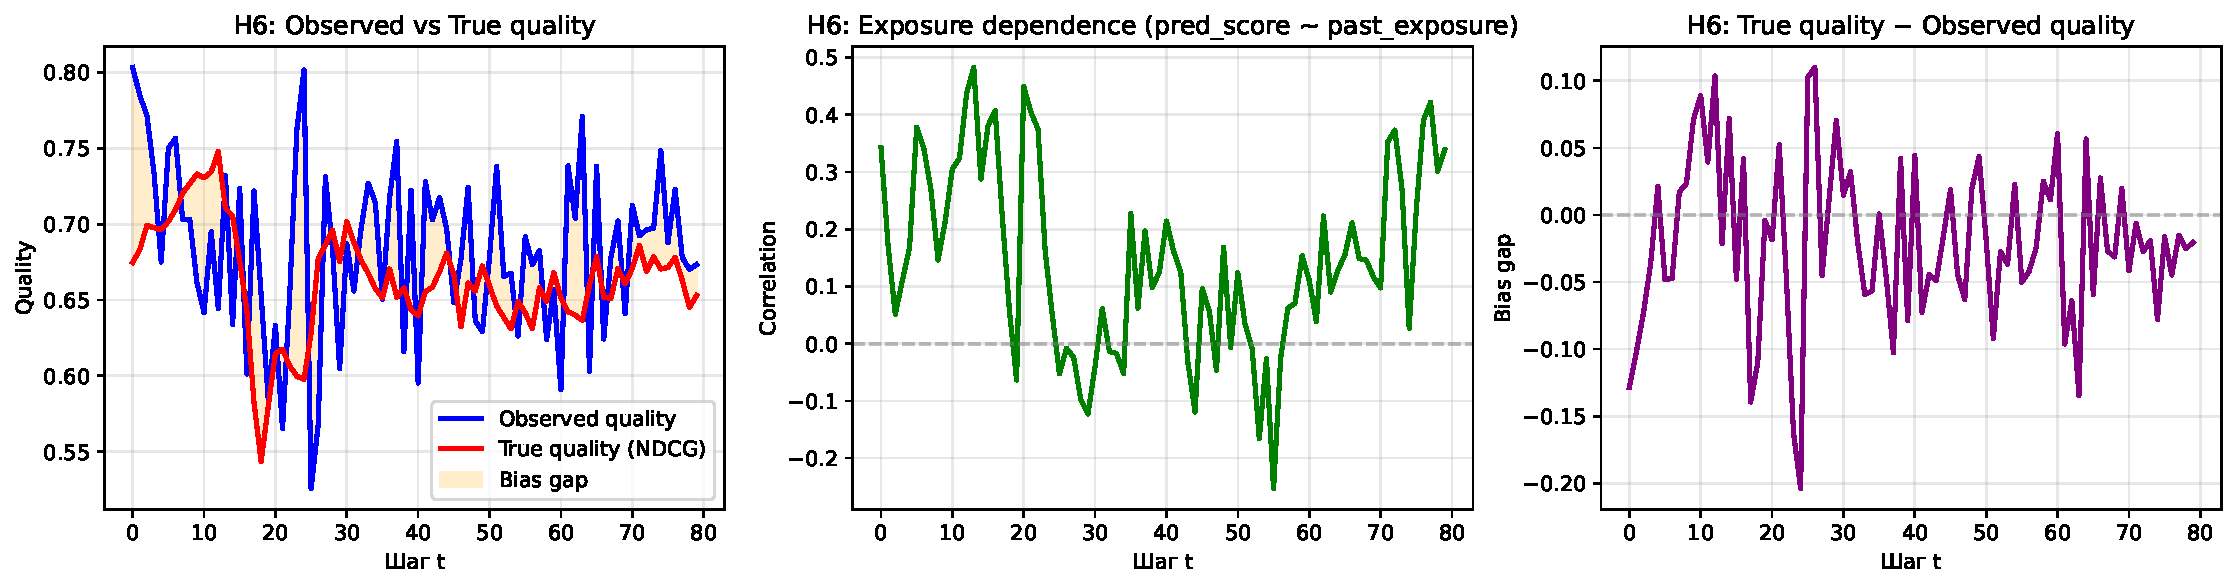
\includegraphics[width=\textwidth]{figures/H6_quality_gap}
    \caption{Наблюдаемое (по логам) и истинное (по вероятностям
    $\theta_t^{ij}$) качество во времени. Наблюдаемое держится выше истинного на
    всём горизонте, что подтверждает
    предложение~\ref{prop:self_reinforcement}.}
    \label{fig:h6_quality}
\end{figure}

\subsection{След петлевого канала в ковариации}
\label{subsec:exp_sensitivity}

Согласно Теореме~\ref{thm:loop}, переобучение оставляет отделимый след в форме
ковариации, а условием его появления служит различимость пользователей
$\lVert J_k\rVert\neq0$. Чтобы выделить этот след, измерялся разрыв между
режимами петли и заморозки при разных классах модели и способах инициализации
(факторный план $2\times3\times4\times30$ запусков). Такая диагностика близка к
идее отделять собственные предпочтения от влияния рекомендателя, но здесь
измеряется не восстановленный отклик, а геометрический след петли в ковариации
~\cite{sinha2016, pagan2023feedbackLoops}.

\begin{figure}[H]
    \centering
    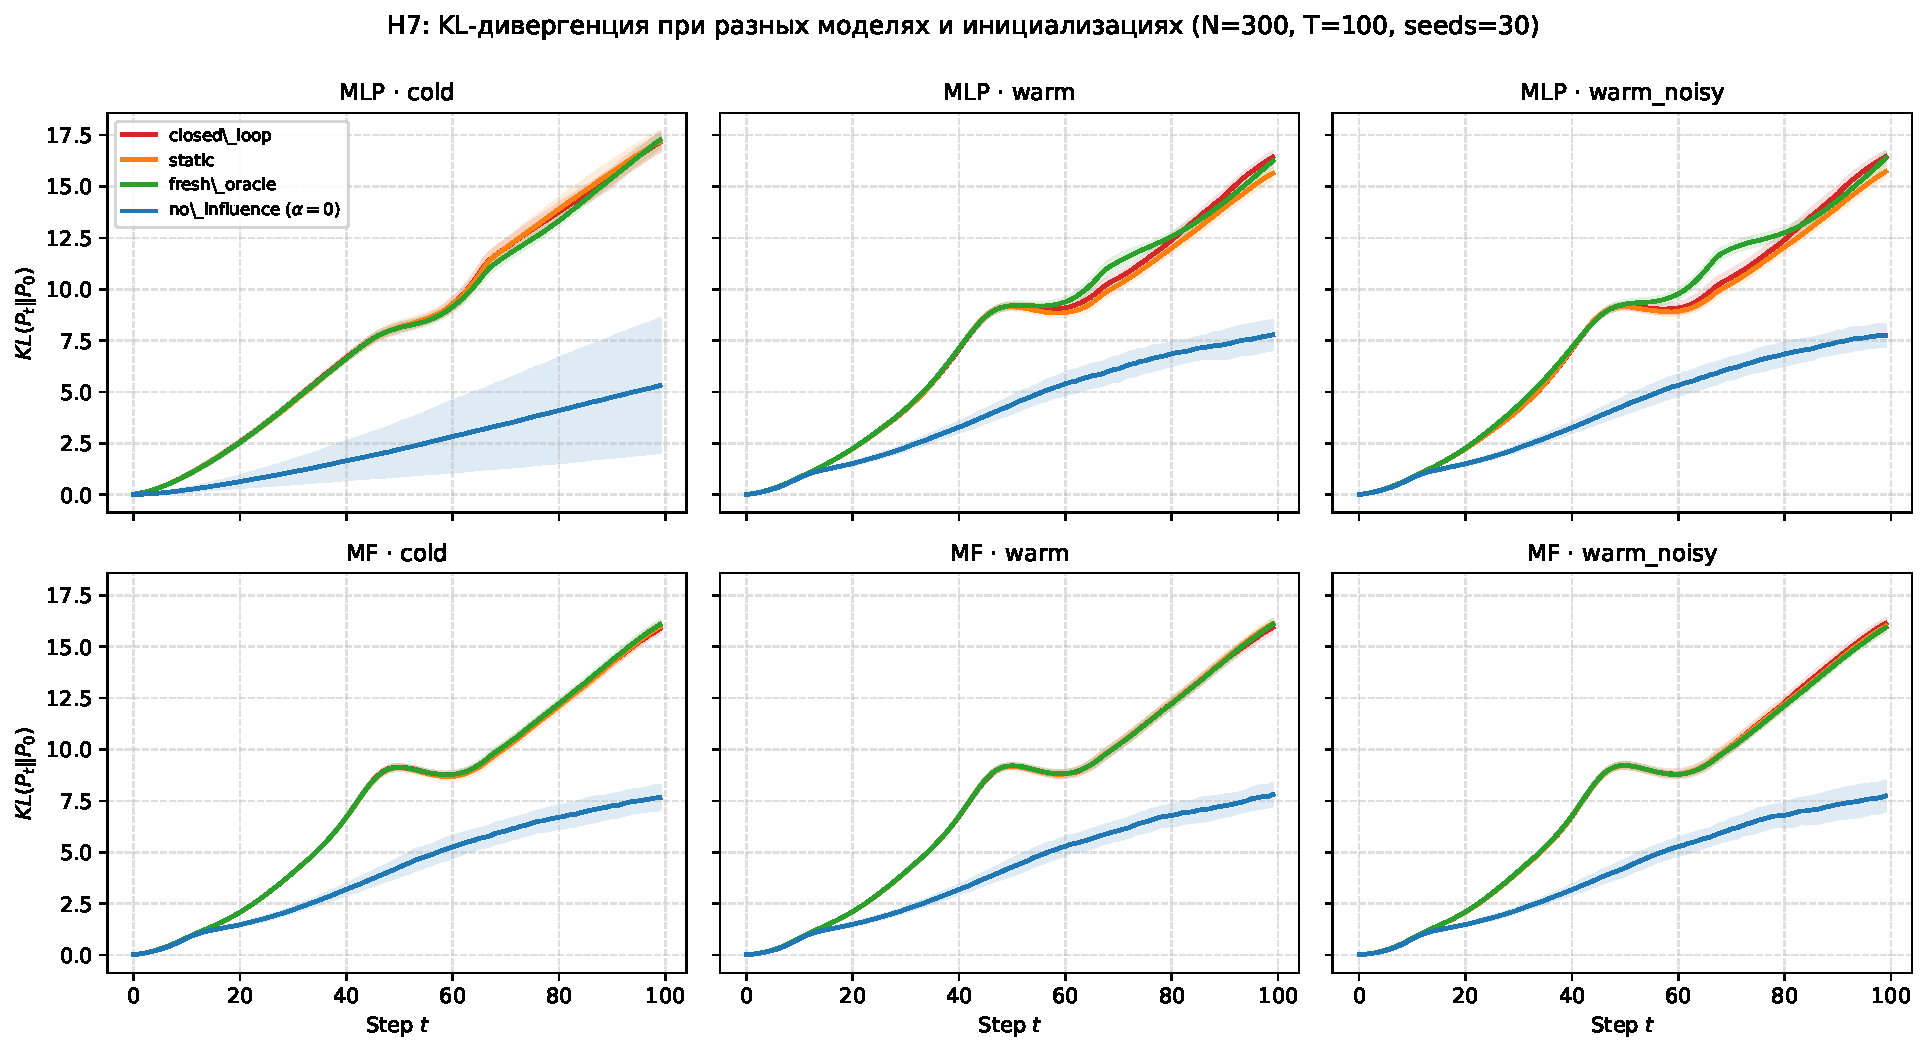
\includegraphics[width=\textwidth]{figures/H7_kl_grid}
    \caption{Разрыв $\mathrm{KL}$ между режимами петли и заморозки по классу
    модели и инициализации. Сигнал петли значим для предобученного MLP, где
    оценка существенно зависит от пользователя ($\lVert J_k\rVert\neq0$), и
    отсутствует при случайной инициализации.}
    \label{fig:h7_kl}
\end{figure}

При предобученной модели (тёплый старт), где $\lVert J_k\rVert\neq0$, разрыв
$\mathrm{KL}$ между петлёй и заморозкой значим и положителен, $+0{,}79$
($95\%$-й доверительный интервал $[0{,}64;0{,}95]$), а разрыв по следу ковариации
составляет $-0{,}16$ (рис.~\ref{fig:h7_kl}): петля даёт более глубокое и иначе
устроенное сжатие. При случайной инициализации, когда оценка почти не зависит от
пользователя, разрыв $\mathrm{KL}$ статистически незначим~--- в полном
согласии с условием активации $\lVert J_k\rVert\neq0$ из
раздела~\ref{subsec:metric}.

Решающую проверку предсказания Теоремы~\ref{thm:loop} о локализации следа даёт
разложение $\mathrm{KL}$ на слагаемое сдвига центра и дисперсионное слагаемое
(таблица~\ref{tab:dispersion}). Весь разрыв между петлёй и заморозкой
сосредоточен в дисперсионном слагаемом ($+0{,}788$), тогда как сдвиг центра
незначим ($+0{,}002$). Это прямо подтверждает, что петля действует на
\emph{ковариацию} предпочтений, а не на положение центров, как и предсказано
обсуждением Теоремы~\ref{thm:loop}.

\begin{table}[H]
    \caption{Разложение разрыва $\mathrm{KL}$ (петля минус заморозка) на слагаемые;
    среднее по $30$ запускам, в скобках $95\%$-й доверительный интервал}
    \label{tab:dispersion}
    \centering
    \begin{tabular}{lc}
        \toprule
        Слагаемое & Разрыв (петля $-$ заморозка) \\
        \midrule
        $\mathrm{KL}$ полное            & $+0{,}789\;[0{,}66;0{,}93]$ \\
        \quad сдвиг центра              & $+0{,}002\;[-0{,}01;0{,}01]$ \\
        \quad дисперсионное слагаемое   & $+0{,}788\;[0{,}66;0{,}93]$ \\
        $\operatorname{tr}\hat\Sigma$   & $-0{,}162\;[-0{,}22;-0{,}11]$ \\
        \bottomrule
    \end{tabular}
\end{table}

Границы активации петлевого канала уточняет эксперимент с варьированием числа
кластеров и баланса их весов (рис.~\ref{fig:h8_K}). При $K=1$ след петли
отсутствует, при $K\ge2$ значим (максимум $+0{,}79$ при $K=3$, далее убывает с
ростом $K$); при сильном перекосе весов сегментов сигнал также исчезает, так как
доминирующий кластер делает популяцию практически одномодальной. Это согласуется
с условием $K\ge2$ из итога главы~\ref{sec:Chapter3}.

\begin{figure}[H]
    \centering
    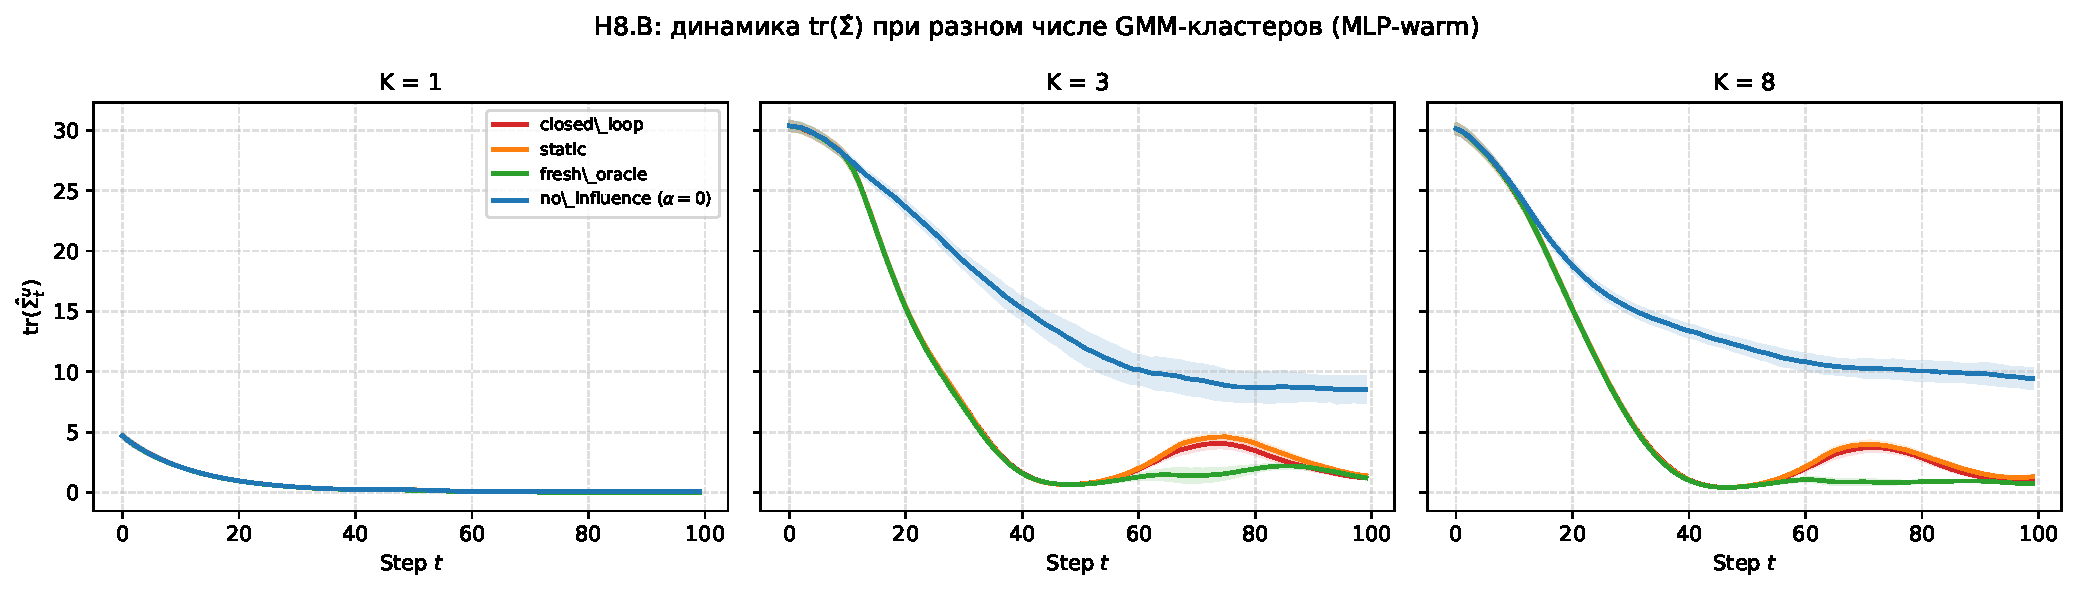
\includegraphics[width=\textwidth]{figures/H8_K_trajectories}
    \caption{Разрыв $\mathrm{KL}$ петля--заморозка в зависимости от числа
    сегментов $K$. Сигнал отсутствует при $K=1$ и значим при $K\ge2$, что
    подтверждает необходимость сегментной структуры для петлевого канала.}
    \label{fig:h8_K}
\end{figure}

% exp: code/experiments/diagnostic/exp_2026-06-15_kl_regularized_retrain.py
\subsection{Прямая проверка оператора переобучения}
\label{subsec:exp_klretrain}

Разложение расхождения локализует след петли в форме ковариации, но проверяет
Теорему~\ref{thm:loop} косвенно~--- через геометрию вкусов, а не через сам
оператор переобучения. Сама теорема опирается на
предположение~\eqref{eq:policy_improve}: переобучение действует как улучшение
политики с регуляризацией Кульбака--Лейблера, заостряя резкость $A_{k,t}$
(предложение~\ref{prop:sharpen}) и тем сужая ковариацию выдачи $C_{k,t}$.
Проверим это предсказание напрямую, заменив в контуре переобучение на сам
оператор~\eqref{eq:policy_improve} и измерив след ковариации показанного. Такая
проверка связывает модель с онлайн-оптимизацией по обратной связи и оптимальным
управлением замкнутой рекомендательной системой~\cite{mariano2026optimalControl,
chandrasekaran2026networkAware}.

В режиме петли кластерная политика инициализируется предобученной моделью
(резкость $A_{k,0}$) и на каждом шаге переобучения перевзвешивается по
Гиббсу, $S_k\leftarrow S_k+\kappa\,\widehat c_{k}$, где $\widehat c_k$~---
средний по кластеру логируемый отклик (смесь истинного отклика и
предсказания модели); в режиме заморозки политика неизменна. Прочие компоненты
контура сохранены, старты режимов совпадают (парный план, $10$ запусков,
$T=100$). Шаг переобучения $\kappa$ варьировался для проверки дозовой
зависимости.

Результаты (таблица~\ref{tab:klretrain}) подтверждают предсказание. Кривизна
отклика неотрицательна~--- предпосылка $H_{k,t}\succeq0$ выполнена во всех
кластерах,~--- а след ковариации выдачи в петле значимо меньше, чем при
заморозке, причём разрыв растёт по модулю с шагом переобучения $\kappa$
(от $-0{,}022$ при $\kappa=5$ до $-0{,}083$ при $\kappa=20$). Это прямо
воспроизводит следствие $\operatorname{tr}C_{k,t}^{\mathrm{closed}}\le
\operatorname{tr}C_{k,t}^{\mathrm{stat}}$ из обсуждения
Теоремы~\ref{thm:loop}: под её собственным оператором переобучение заостряет
выдачу, и тем сильнее, чем интенсивнее переобучение.

\begin{table}[H]
    \caption{Прямая проверка оператора переобучения~\eqref{eq:policy_improve}:
    разрыв следа ковариации выдачи $\operatorname{tr}C$ между режимами петли и
    заморозки; среднее по $10$ запускам, в скобках $95\%$-й доверительный интервал}
    \label{tab:klretrain}
    \centering
    \begin{tabular}{lc}
        \toprule
        Величина & Значение \\
        \midrule
        Кривизна отклика $H_{k,t}\succeq0$ (доля кластеров) & $100\%$ \\
        $\operatorname{tr}C$, петля $-$ заморозка ($\kappa=5$)  & $-0{,}022\;[-0{,}027;-0{,}017]$ \\
        $\operatorname{tr}C$, петля $-$ заморозка ($\kappa=20$) & $-0{,}083\;[-0{,}103;-0{,}064]$ \\
        \bottomrule
    \end{tabular}
\end{table}

Проверка относится к идеализированному оператору~\eqref{eq:policy_improve}. В
промышленных системах переобучение минимизирует существенно более сложную
функцию потерь~--- бинарную кросс-энтропию глубокой модели и её варианты,~---
оператор которой не сводится к чистому улучшению политики, и заострение выдачи в
таком режиме достигается труднее. Поэтому приведённый результат подтверждает
механизм Теоремы~\ref{thm:loop} в рамках её модельного допущения о форме
переобучения, оставляя количественную силу эффекта в реальных архитектурах
предметом дальнейшего изучения.

% exp: code/experiments/diagnostic/exp_2026-06-15b_kl_risk_gap.py
\subsection{Рост расхождения и надёжность офлайн-метрик}
\label{subsec:exp_klgap}

Предложение~\ref{prop:pinsker} ограничивает разрыв между наблюдаемым и истинным
качеством расхождением $\overline{\mathrm{KL}}_t$ между загрязнённым и истинным
откликом. Проверим, как $\overline{\mathrm{KL}}_t$ ведёт себя в контуре и
выполняется ли граница. На каждом шаге по показанным парам (распределение показов $\mu_t$)
измерялись $\overline{\mathrm{KL}}_t$, завышение метрики
$Q^{\mathrm{obs}}-Q^{\mathrm{true}}$ (наблюдаемый и истинный CTR показанного) и
граница Пинскера; режимы петли, заморозки и без влияния, $8$ запусков, $T=100$.
Такой эксперимент важен именно для офлайн-оценивания: стандартные метрики
ранжирования зависят от того, какие пары пользователь--объект были показаны, и
поэтому могут терять связь с истинной полезностью при смещённом распределении показов
~\cite{krichene2020, stoecker2025biasMitigation}.

\begin{figure}[H]
    \centering
    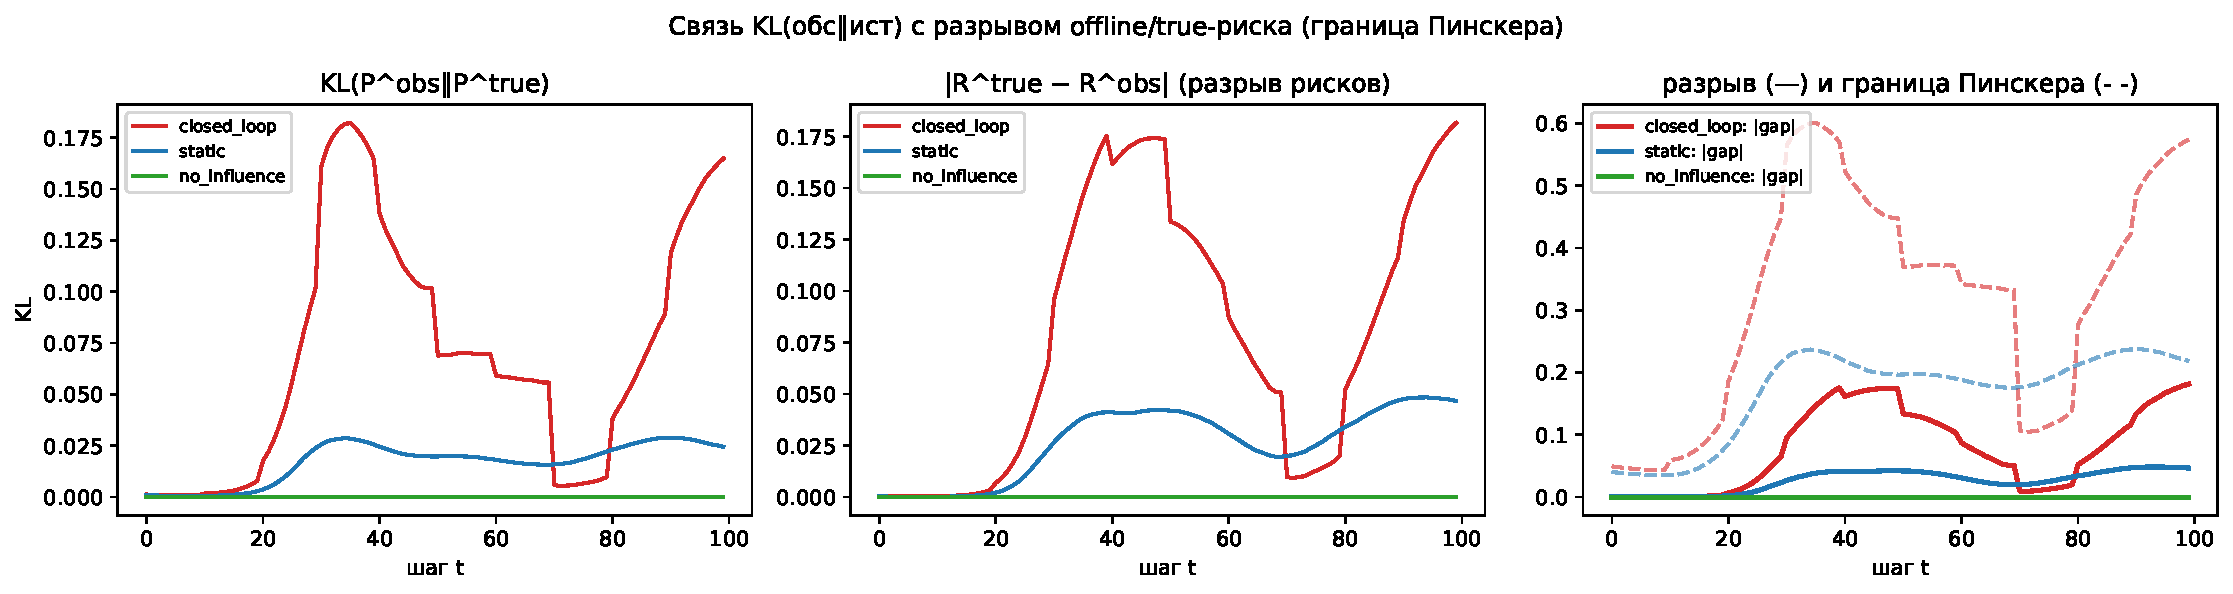
\includegraphics[width=\textwidth]{figures/diagnostic/DIAG_kl_risk_gap}
    \caption{Расхождение $\overline{\mathrm{KL}}_t$ между наблюдаемым и истинным
    откликом (слева), разрыв качества $|Q^{\mathrm{obs}}-Q^{\mathrm{true}}|$ (в
    центре) и его сравнение с границей Пинскера (справа, штрих) по трём режимам. В
    режиме петли расхождение и разрыв растут со шагом контура; в режиме без влияния
    ($\alpha=0$) загрязнения нет.}
    \label{fig:kl_risk_gap}
\end{figure}

Результаты (рис.~\ref{fig:kl_risk_gap}, таблица~\ref{tab:klgap}) подтверждают
предсказание. В режиме петли $\overline{\mathrm{KL}}_t$ растёт со шагом контура
(с почти нуля до $0{,}17$), завышение метрики увеличивается синхронно~--- до
$+0{,}18$ (наблюдаемый CTR $0{,}92$ против истинной релевантности $0{,}74$),~--- и
величина разрыва тесно следует за $\sqrt{\overline{\mathrm{KL}}_t}$ (коэффициент
корреляции $0{,}93$). Граница Пинскера выполняется на каждом шаге. Эффект
специфичен для переобучения: при заморозке рост $\overline{\mathrm{KL}}$ примерно
впятеро слабее (разрыв петля$-$заморозка по $\overline{\mathrm{KL}}$ значим,
$+0{,}14$, доверительный интервал $[0{,}13;0{,}15]$), а в режиме без влияния
загрязнения нет и $\overline{\mathrm{KL}}\equiv0$.

\begin{table}[H]
    \caption{Расхождение наблюдаемого и истинного отклика и разрыв качества на
    горизонте $t=T$; среднее по $8$ запускам}
    \label{tab:klgap}
    \centering
    \begin{tabular}{lcc}
        \toprule
        Режим & $\overline{\mathrm{KL}}_T$ & $|Q^{\mathrm{obs}}-Q^{\mathrm{true}}|_T$ \\
        \midrule
        \texttt{closed\_loop}  & $0{,}165$ & $0{,}182$ \\
        \texttt{static}        & $0{,}024$ & $0{,}047$ \\
        \texttt{no\_influence} & $0{,}000$ & $0{,}000$ \\
        \bottomrule
    \end{tabular}
\end{table}

По мере работы контура наблюдаемое качество расходится с истинным не быстрее, чем
позволяет $\overline{\mathrm{KL}}_t$, и поскольку переобучение на собственных
логах увеличивает это расхождение, офлайн-метрики перестают быть надёжным
индикатором реальной пользы~--- в количественном согласии с
Предложением~\ref{prop:pinsker}.

\subsection{Эксперименты на реальных данных}
\label{subsec:exp_real}

Для проверки переносимости выводов использован набор данных
\texttt{MovieLens-20M}~\cite{movielens20m}. В первой постановке синтетический
генератор пользователей заменён эмпирическим, восстановленным по матрице оценок
($500\times500$ после фильтрации, $d=16$, матричная факторизация, $3$ запуска);
прочие компоненты контура сохранены. Результаты воспроизводят синтетические:
$\operatorname{tr}\hat\Sigma$ в петле равен $0{,}174$ против $0{,}339$ в
\texttt{no\_influence}, а $\mathrm{KL}$ составляет $34{,}5$ против $19{,}7$
(разрыв $1{,}75$ раза), причём с более выраженным разделением режимов
(рис.~\ref{fig:real_ml}).
Использование MovieLens здесь не предполагает, что реальные логи являются
нейтральной выборкой предпочтений: напротив, именно такие исторические данные
мотивируют методы деконволюции и каузальной коррекции петли обратной связи
~\cite{sinha2016, chaney2018, krauth2022}.

\begin{figure}[H]
    \centering
    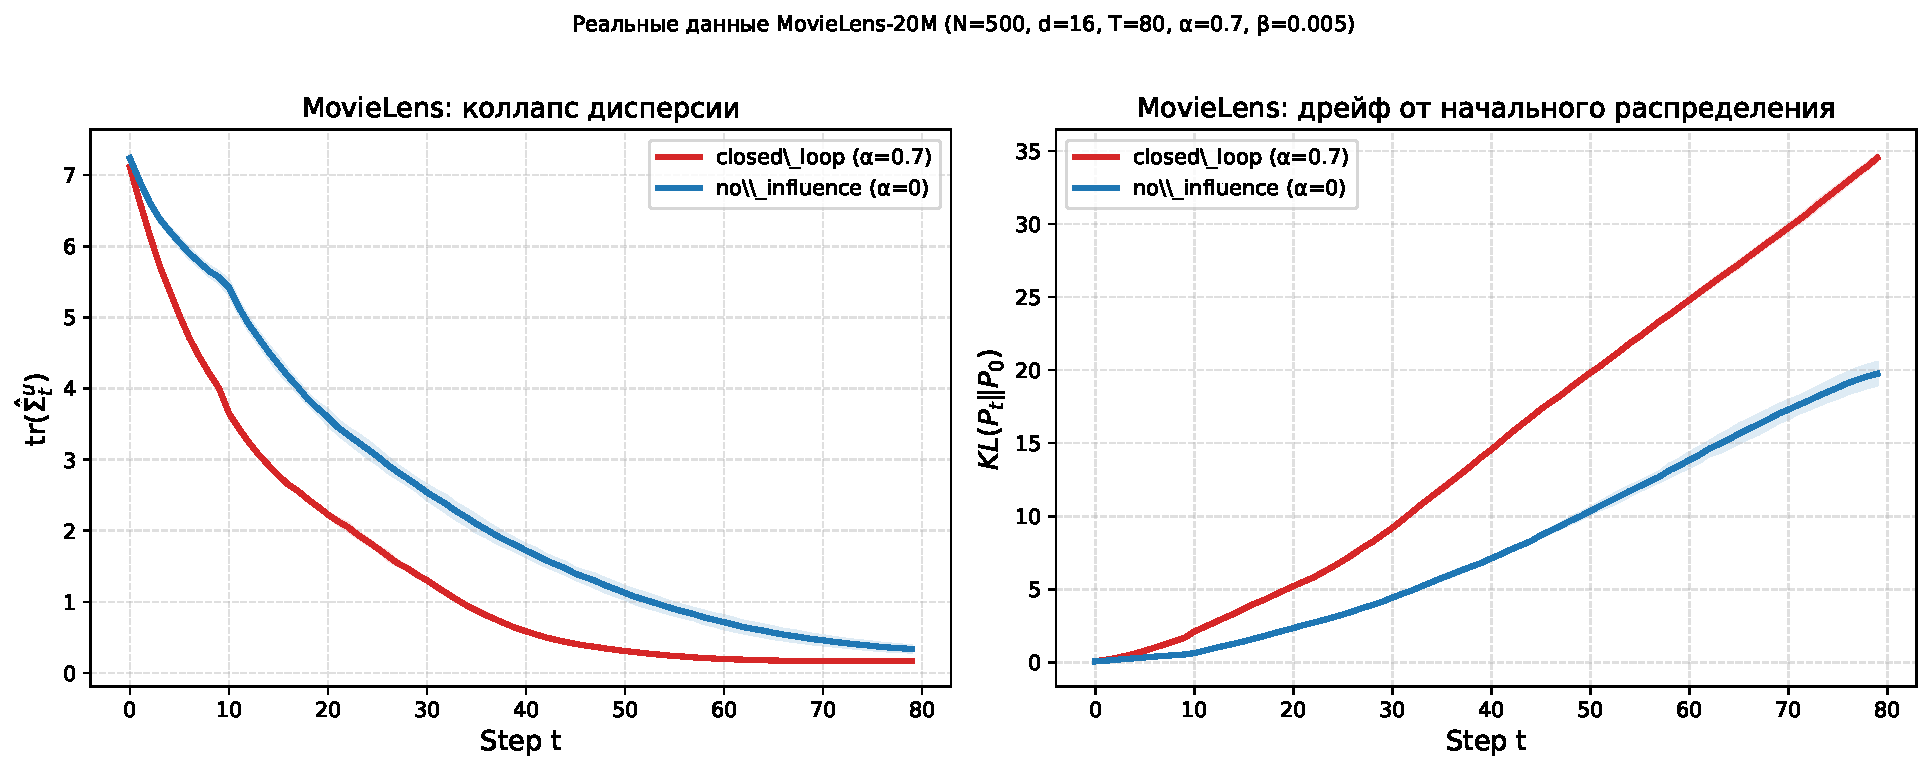
\includegraphics[width=\textwidth]{figures/real_data_movielens}
    \caption{Динамика $\mathrm{KL}(P_t\Vert P_0)$ и $\operatorname{tr}\hat\Sigma_t$
    на \texttt{MovieLens-20M} с эмпирическим генератором пользователей. Эффект
    воспроизводится вне синтетической среды.}
    \label{fig:real_ml}
\end{figure}

Во второй постановке коллапс наблюдается непосредственно в распределении
рекомендаций, без обращения к дрейфу эмбеддингов: модель в режиме петли
дообучается на собственных списках top-$L$ ($3000\times3000$, $d=32$, $L=10$,
$17$ квартальных окон). Покрытие каталога падает с $0{,}68$ до $0{,}24$, а
коэффициент Джини частот рекомендаций растёт с $0{,}67$ до $0{,}91$
(рис.~\ref{fig:collapse_direct}); в контрольном режиме без переобучения изменения
отсутствуют. Спустя моделируемый год система рекомендует втрое меньшую долю
каталога, что подтверждает выводы на уровне работы системы.

\begin{figure}[H]
    \centering
    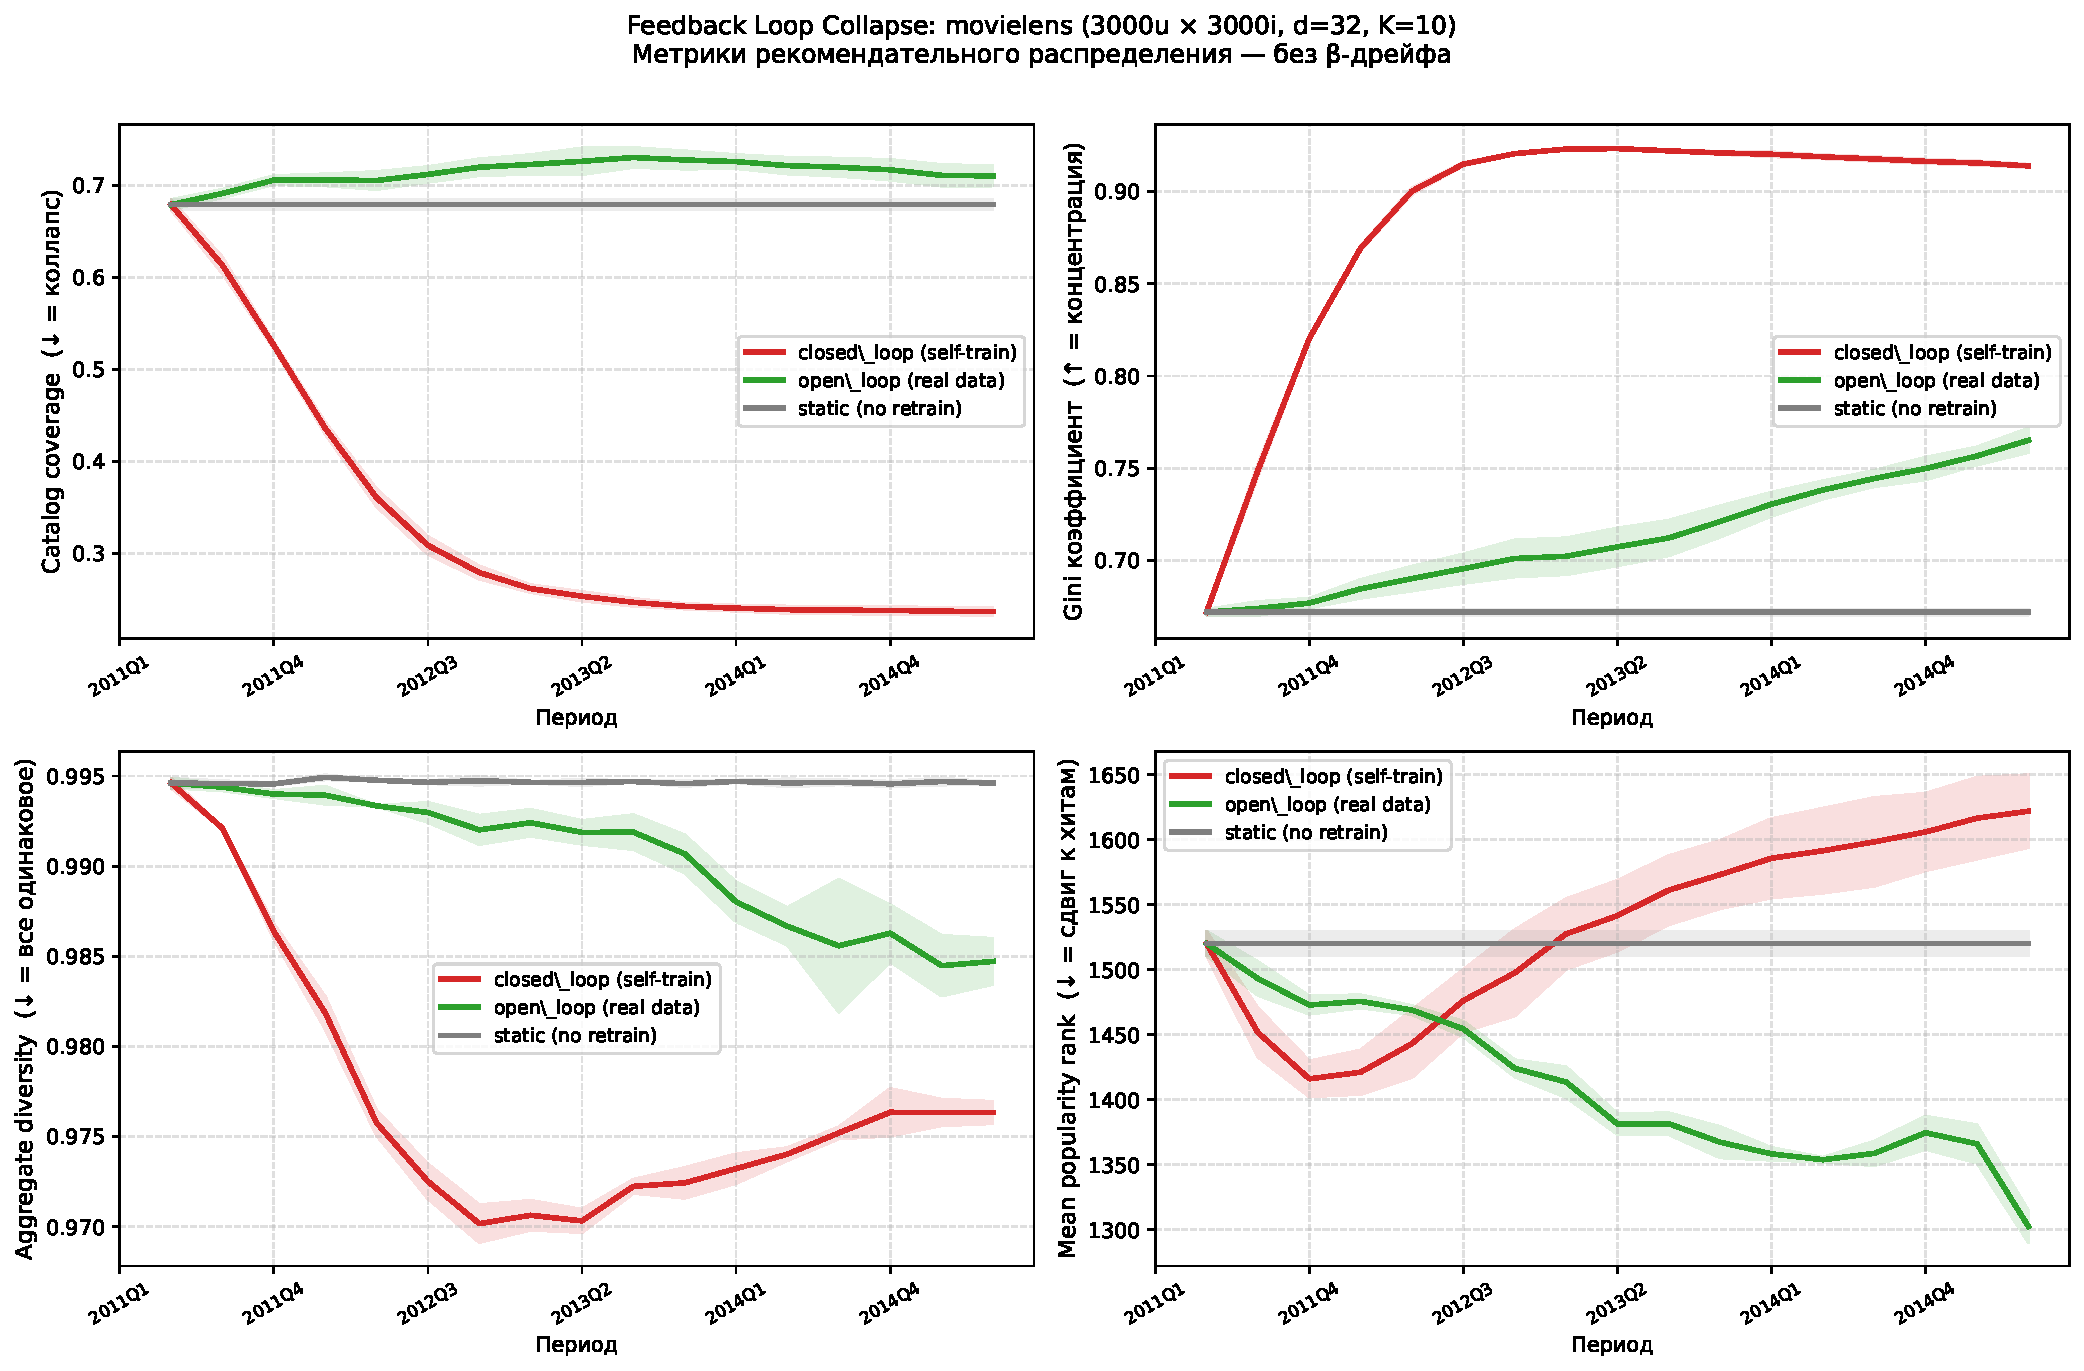
\includegraphics[width=\textwidth]{figures/collapse_direct_movielens}
    \caption{Прямое измерение стягивания распределения рекомендаций на
    \texttt{MovieLens-20M}: покрытие каталога, коэффициент Джини и разнообразие по
    трём режимам. В режиме петли покрытие падает более чем вдвое; контрольные
    режимы стабильны.}
    \label{fig:collapse_direct}
\end{figure}

Третья постановка проверяет само допущение о дрейфе предпочтений~\eqref{eq:drift}:
до сих пор сила дрейфа $\beta$ задавалась как параметр модели и из данных не
измерялась. В пространстве жанровых тегов \texttt{genome} ($1128$ признаков,
выведенных из содержания фильмов и независимых от поведенческих эмбеддингов;
сжато методом главных компонент до $20$ измерений) для каждого пользователя
строилась временная траектория центроидов потребления по последовательным окнам
просмотров. К ней применялась модель пространства состояний типа «случайное
блуждание с шумом», в которой стационарность потребления отвечает $\beta=0$, а
отношение дисперсии дрейфа к дисперсии внутриоконного шума даёт оценку
$\hat\beta=\sigma_\nu/\sigma_\varepsilon$. На $9{,}9$~млн положительных оценок
(порог $\ge 4$, $47{,}9$~тыс. пользователей) оценка дрейфа в $15$--$21$ раз
превосходит контрольное значение, полученное при перестановке порядка окон, по
всем $20$ компонентам, что свидетельствует о значимой нестационарности
предпочтений во времени. Полученная верхняя граница по наблюдательным данным на силу
дрейфа за один отклик составляет порядка $0{,}04$--$0{,}08$, внутри которой
используемое в симуляции значение $\beta=0{,}005$ оказывается консервативным.
Поскольку без экзогенной вариации показов рекомендательно-индуцированный
дрейф неотделим от автономной эволюции вкусов, эта оценка является верхней
границей; её каузальное уточнение намечено в главе~\ref{sec:Chapter6}.

\subsection{Сводка: теория и эксперимент}
\label{subsec:exp_summary}

Таблица~\ref{tab:theory_exp} сопоставляет теоретические утверждения с их
численным подтверждением. Все ключевые предсказания обеих теорем подтверждены,
в том числе на реальных данных.

\begin{table}[H]
    \caption{Соответствие теоретических утверждений и эксперимента}
    \label{tab:theory_exp}
    \centering
    \begin{tabular}{p{6.2cm}p{3.2cm}p{4.2cm}}
        \toprule
        Утверждение & Эксперимент & Результат \\
        \midrule
        Предложение~\ref{prop:self_reinforcement}: наблюдаемое выше истинного &
        качество, рис.~\ref{fig:h6_quality} & $0{,}69\!\to\!0{,}66$ ниже
        $0{,}75\!\to\!0{,}69$ \\
        Теорема~\ref{thm:beta}: нет стягивания при $\beta=0$ &
        варьирование $\beta$ & $\operatorname{tr}\hat\Sigma\approx30$ \\
        Следствие~\ref{cor:universal}: универсальность по режиму &
        режимы \texttt{static}/\texttt{oracle} & спад $\approx97\%$ \\
        Теорема~\ref{thm:beta}: монотонность по $\alpha\rho$ &
        фазовая диаграмма & $0{,}27\to0{,}02$ \\
        Теорема~\ref{thm:beta}: глобальный аттрактор &
        $23$ инициализации & все $\to0$ \\
        Теорема~\ref{thm:loop}: след петли при $\lVert J_k\rVert\neq0$ &
        тёплый старт MLP & $\operatorname{tr}$ $-0{,}16$, $\mathrm{KL}$ $+0{,}79$ \\
        Теорема~\ref{thm:loop}: след в ковариации, не в центре &
        разложение $\mathrm{KL}$ & дисп. $+0{,}79$, центр $+0{,}00$ \\
        Условие $K\ge2$ & варьирование $K$ & $K{=}1$: нет; $K\ge2$: есть \\
        Перенос на реальные данные & \texttt{MovieLens-20M} &
        $\operatorname{tr}$ $0{,}17$ vs $0{,}34$ \\
        \bottomrule
    \end{tabular}
\end{table}
